\chapter{Theoretischer Hintergrund}
Im folgenden Kapitel werden die theoretischen Grundlagen für diese Arbeit erläutert, um ein Verständnis für die verwendeten Begriffe und Technologien zu schaffen. Zunächst wird ein kurzer Überblick über die \ac{OCR} gegeben. Anschließend werden die Grundlagen der Transformer-Modelle erläutert. Des Weiteren werden die Details des \ac{Donut} genauer betrachtet, um ein Verständnis für die Funktionsweise des Modells im Vergleich zu herkömmlichen Methoden zu schaffen.

\section{Grundlagen von OCR}
Dieser Abschnitt betrachtet die grundlegende Funktionsweise und die Anwendungsbereiche von OCR-Systemen, da auch heute noch die meisten Modelle der Dokumentenverarbeitung auf eine OCR für den textuellen Input angewiesen sind (siehe dazu bspw. LayoutLM3\footcites[Vgl. dazu ausführlich][]{huang_layoutlmv3_2022}, ERNIE\footcites[Vgl. dazu ausführlich][]{peng_ernie-layout_2022}, FastStrucText\footcites[Vgl. dazu ausführlich][]{zhai_fast-structext_2023} etc.). Der Abschnitt bietet einen grundlegenden Überblick über das Thema. Auf ein tieferes Verständnis und eine detaillierte Betrachtung der Funktionsweise von OCR-Systemen wird in dieser Arbeit nicht eingegangen, da der Fokus auf der Anwendung von Transformer-Modellen im Bereich der Dokumentenverarbeitung liegt. Dennoch darf die Relevanz von OCR-Systemen nicht unterschätzt werden, da sie in vielen \ac{SOTA}-Modellen immer noch als Basis für die Textextraktion dienen. 

Häufig liegen Informationen in handschriftlicher oder gedruckter Form vor. Diese Informationen können durch Scans als Bilder in Computern gespeichert werden, jedoch ist die Weiterverarbeitung der Informationen schwierig. Das System kann nicht ohne weiteres auf den Text in den erfassten Bildern zugreifen, bzw. diesen lesen. Das Ziel von OCR ist es, Text aus Bildern zu extrahieren. OCR-Systeme sind in der Lage, Text aus gescannten Dokumenten, Fotos oder anderen Bildern zu extrahieren und in maschinenlesbaren Text umzuwandeln. In einem solchen Format können die Informationen weiterverarbeitet und analysiert werden. Somit ermöglicht es OCR einer Maschine, Texte automatisch zu erkennen.\footcites[Vgl.][S. 244]{hamad_detailed_2016}

Die Funktionsweise von OCR-Systemen kann in sechs Phasen unterteilt werden. Diese Phasen umfassen die Vorverarbeitung, die Segmentierung, die Normalisierung, die Merkmalsextraktion, die Klassifikation und die Postverarbeitung. Das Ziel der Vorverarbeitung ist es, das Eingabebild zu verbessern und zu bereinigen um es für eine bessere Erkennung vorzubereiten. Dazu gehören Techniken wie Rauschreduzierung, Kontrastanpassung und Skalierung. In der Segmentierung wird das Bild in kleinere Einheiten aufgeteilt, typischerweise in Zeilen, Wörter oder einzelne Zeichen. Eine präzise Segmentierung ist für die Genauigkeit der nachfolgenden Erkennungsprozesse von entscheidender Bedeutung, da sie bestimmt, wie Textelemente voneinander getrennt und identifiziert werden. Sie stellt die kritische und maßgebliche Komponente eines OCR-Systems dar. Die Normalisierung ist der Prozess, bei dem die Segmentierungsergebnisse in eine standardisierte Form gebracht werden. Nach der Segmentierung werden die extrahierten Textsegmente normalisiert, um eine einheitliche Größe und Ausrichtung zu gewährleisten. Diese Standardisierung ist notwendig, um die Vielfalt der Textdarstellungen zu reduzieren und die Effektivität der Merkmalsextraktion und Klassifikation zu verbessern. In der Merkmalsextraktionsphase extrahiert das System relevante Merkmale von Objekten oder Alphabeten. In dieser Phase werden aus den normalisierten Textsegmenten charakteristische Merkmale extrahiert, die zur Unterscheidung zwischen verschiedenen Zeichen oder Wörtern dienen. Diese Merkmale können Form, Größe, Strichrichtung und andere visuelle Eigenschaften umfassen, die zur Erstellung von Merkmalsvektoren verwendet werden. In der Klassifikationsphase werden die Eingaben unterschiedlichen Klassen zugeordnet wobei jede Klasse einem bestimmten Zeichen oder Wort entspricht.\footcites[Vgl.][S. 244]{hamad_detailed_2016} Beispielsweise wird in der Klassifikationsphase die Rechnungsnummer einer Klasse \emph{Invoice-Nr.} zugeordnet und das Datum der Klasse \emph{Date}. Es gibt diverse Werkzeuge, um die Klassifikation durchzuführen. Laut Dongre u.a. ist das \emph{Character Classification Problem} verwandt mit der heuristischen Logik, da Menschen Zeichen und Dokumente durch Erfahrung und Lernen erkennen können. Da Neuronale Netze ebenfalls von heuristischer Natur sind, sollten sie sich besonders gut für solche Probleme eignen. \footcites[Vgl.][S. 11]{dongre_review_2010} Hier bleibt jedoch unbeachtet, dass die Eignung auch von der Qualität des Netzes selbst abhängt, welche wiederrum von der Qualität der Trainingsdaten abhängig ist.\footcites[Vgl.][S. 851]{kavzoglu_increasing_2009} Daher eignet sich das Neuronale Netz als Klassifikator nur dann besonders gut, wenn die Trainingsdaten von hoher Qualität sind und das Netz in der Klassifikation eine hohe Genauigkeit aufweist. Die Postverarbeitung dient der Feinabstimmung und Korrektur der Erkennungsergebnisse. Durch den Einsatz von Sprachmodellen und lexikalischen Datenbanken werden Tippfehler korrigiert und die Kohärenz des erkannten Textes verbessert. Die Postverarbeitung spielt eine wichtige Rolle bei der Steigerung der Gesamtgenauigkeit des OCR-Systems, indem sie kontextuelle Hinweise und linguistisches Wissen nutzt.\footcites[Vgl.][S. 246 f.]{hamad_detailed_2016} Hier wird das zuvor genannte \ac{BERT} eingesetzt, um die Genauigkeit der OCR-Systeme zu verbessern.\footcites[Vgl.][S. 335 f.]{nguyen_neural_2020}

Für eine hohe Qualität und Genauigkeit der Zeichenerkennung erwarten OCR-Systeme eine hohe Qualität der Eingabebilder. Die Qualität der Eingabebilder ist ein entscheidender Punkt für die Genauigkeit der Zeichenerkennung. Einige Faktoren stellen Herausforderungen für OCR dar, darunter die Szenenkomplexität, ungleiche Beleuchtungsbedingungen, Verzerrungen, Unschärfe und Abbau, Aspektverhältnisse, die Kippung, die Schriftart und mehrsprachige Umgebungen.\footcites[Vgl.][S. 245]{hamad_detailed_2016} Die Herausforderungen erfordern fortgeschrittene Algorithmen und Techniken, einschließlich maschinellem Lernen und künstlicher Intelligenz, um die Erkennungsrate zu verbessern. Diese Herausforderungen versucht das Donut-Modell zu überwinden, indem es auf Transformer-Modellen basiert und somit die Limitierungen von OCR-Systemen umgeht.\footcites[Vgl.][S. 1]{kim_ocr-free_2021} Um die Ergebnisse von OCR-Systemen zu verbessern werden in der Literatur verschiedene Ansätze vorgeschlagen. Nguyen et. al. schlagen die Verwendung von BERT vor. Als kontextbasiertes Sprachmodell kann BERT die Genauigkeit der OCR-Systeme verbessern, indem es die Kontextinformationen der Wörter berücksichtigt. Die Autoren zeigen, dass BERT die Genauigkeit der OCR-Systeme durch Fehlererkennung und Korrektur verbessern kann.\footcites[Vgl.][S. 335 f.]{nguyen_neural_2020} BERT und seine Derivate werden noch heute in vielen \ac{SOTA}-Modellen für die Textextraktion verwendet.\footcites[Vgl. dazu ausführlich][S. 4084 ff.]{huang_layoutlmv3_2022} \footcites[Vgl. dazu ausführlich][S. 2 ff.]{garncarek_lambert_2020}

Die Anwendungsbereiche der OCR sind vielfältig. Sie reichen von der Digitalisierung von Dokumenten in der Rechtsbranche über die Verarbeitung von Checks in Banken bis ins Gesundheitswesen. Der für diese Arbeit relevante Verwendungszweck ist die Verarbeitung von Rechnungen. OCR-Systeme werden in vielen Organisationen eingesetzt, um Rechnungen zu digitalisieren und diese so weiterzuverarbeiten.\footcites[Vgl.][S. 247 f.]{hamad_detailed_2016}

\section{Transformer-Modelle}
Im Folgenden soll ein Verständnis für die Transformer-Modelle geschaffen werden, welche wiederum die Grundlage für Donut bilden. Dabei werden zunächst die Herkunft und Relevanz der Transformer-Modelle (folgend auch Transformer genannt) erläutert. Anschließend wird die Funktionsweise des Systems genauer betrachtet. Dabei werden Schlüsselkonzepte wie die Aufmerksamkeit und das Positional Encoding sowie die Architektur der Modelle erläutert. Die mathematischen Grundlagen werden hierbei nicht betrachtet, da sie den Umfang dieser Arbeit übersteigen. Im Gegensatz zum Großteil der Fachliteratur fokussiert sich dieser Abschnitt jeweils darauf, warum sich eine Komponente/Mechanismus im Modell befindet, welche Funktionen sie erfüllt und welche Vorteile diese mit sich bringt. Seit der Einführung der Transformer in 2017 durch Vaswani et al. \footcites{vaswani_attention_2017} sind diese zum de facto Standard für eine Reihe verschiedener \ac{NLP} Aufgaben geworden. \ac{NLP} ist ein Teilbereich der Informatik, welcher es Computern ermöglichen soll, ähnlich wie Menschen, Sprache auf eine \emph{natürliche} Art und Weise zu verstehen. Typischerweise referenziert dies Aufgaben wie das Verstehen von Gefühlen in Texten, die Spracherkennung und das Generieren von Antworten auf Fragen. \footcites[Vgl.][S. 1]{beysolow_ii_applied_2018} Mittlerweile werden Transformer in den bekanntesten und meist genutzten Modellen der Welt verwendet, darunter BERT und GPT. \footcites[Vgl.][S. 1]{tunstall_natural_2022} Die beachtliche Leistungsfähigkeit der Transformer zeigt sich in den Benutzerzahlen von ChatGPT (ein Chatbot von OpenAI, welcher auf den Transformer-Modellen basiert). Innerhalb von fünf Tagen nach der Veröffentlichung des Modells hatte ChatGPT bereits eine Millionen Nutzer. Im Vergleich dazu brauchte Instagram 2,5 Monate, um die gleiche Anzahl an Nutzern zu erreichen. \footcites[Vgl.][]{buchholz_infographic_2023} Den Status quo, vor der Entwicklung der Transformer, bildeten die \ac{RNN} und \ac{LSTM} Modelle. Transformer erzielen sowohl in der Leistungsfähigkeit als auch in den Trainingskosten bessere Ergebnisse als seine Vorgänger. \footcites[Vgl.][S. 1]{tunstall_natural_2022}

\subsection{Encoder-Decoder Architektur}
Das ursprüngliche Transformer-Modell, präsentiert von Vaswani et al. in 2017, basiert auf einer \emph{Encoder-Decoder} Architektur. Diese Architektur eignet sich besonder gut für Situationen, in welchen es sich sowohl bei der Ein- als auch der Ausgabe um Sequenzen handelt. Der Encoder wandelt die Eingabe von einer Sequenz in eine numerische Repräsentation um, welche häufig als \emph{last hidden state} bezeichnet wird. Dieser Zustand wird dann in den Decoder übergeben, welcher die Ausgabesequenz generiert. \footcites[Vgl.][S. 3 ff.]{tunstall_natural_2022} Die grundlegende Architektur des Transformer-Modells wird in Abb. \ref{fig:transformer-architecture} dargestellt. 

\begin{figure}[h]
    \centering
    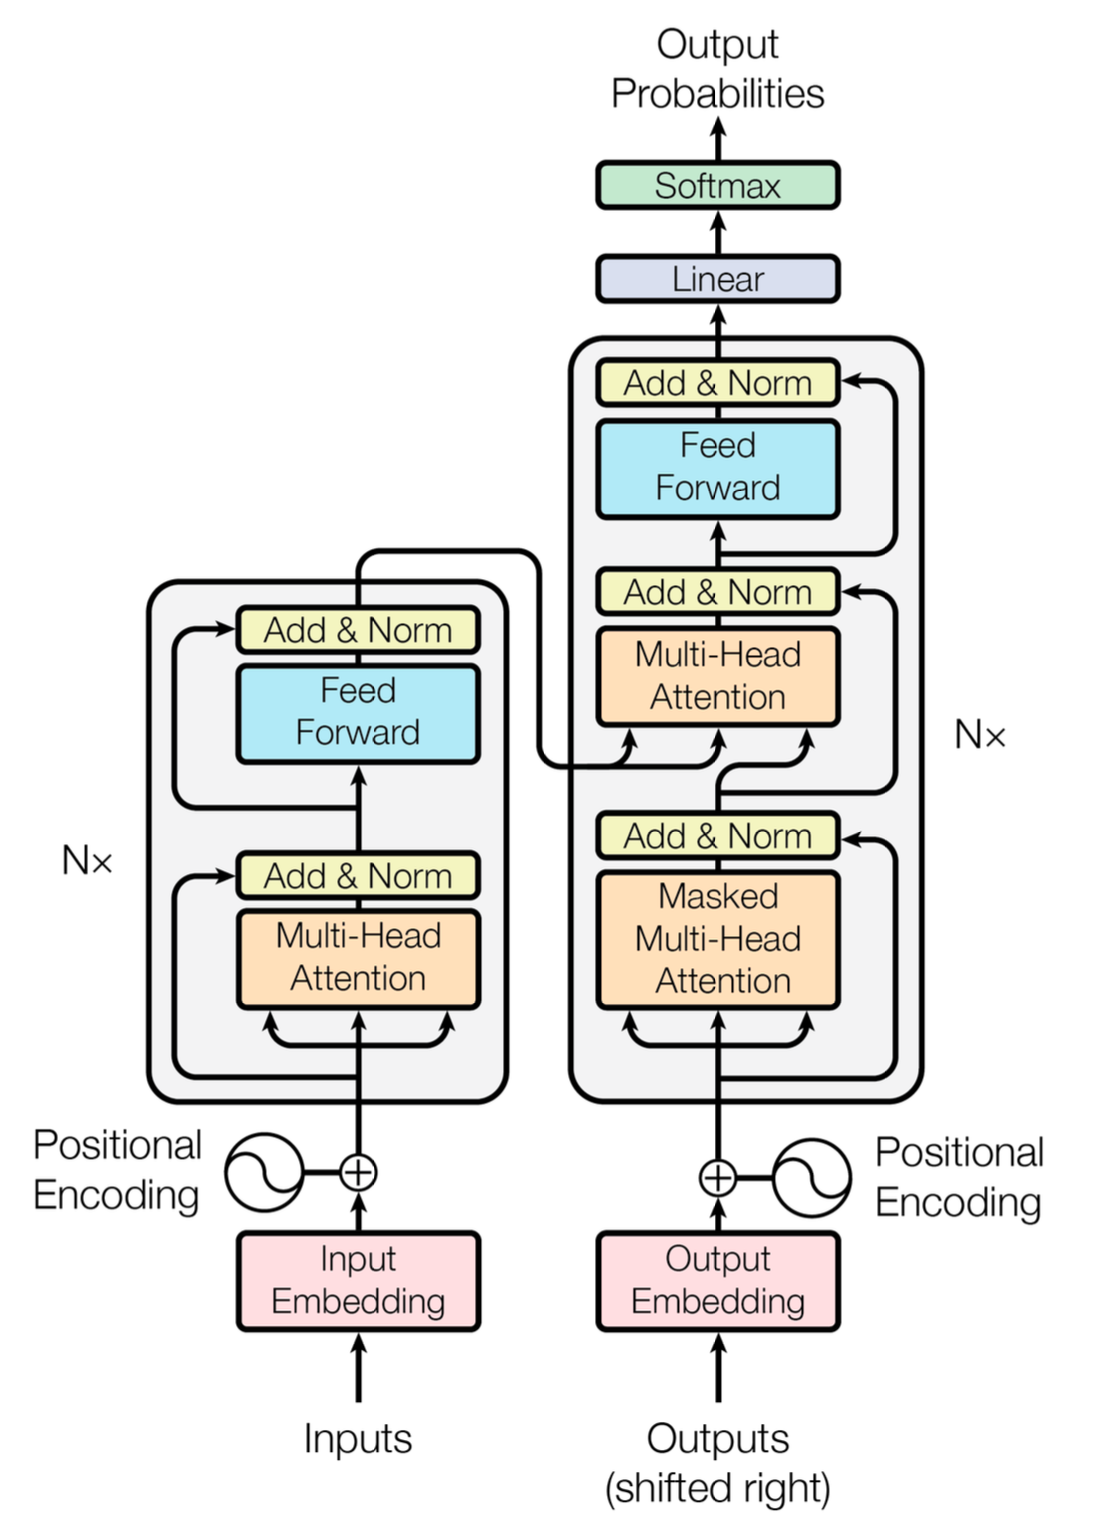
\includegraphics[height=100mm]{graphics/architecture.png}
    \caption[Architektur des Transformer-Modells]{Architektur des Transformer-Modells \footnotemark}
    \label{fig:transformer-architecture}
\end{figure}

\footnotetext{Entnommen aus: \cite{vaswani_attention_2017}, S. 3} %FIXME: Fußnote sitzt noch auf der vorherigen Seite...
Der linke Block beschreibt dabei den Encoder während der rechte Block den Decoder darstellt. Es werden mehrere Schichten dieser Blöcke gestapelt, was durch das \emph{Nx} gekennzeichnet wird. Das Modell nach Vaswani et al. verwendet sechs Schichten für den Encoder und sechs Schichten für den Decoder. Der Encoder-Block besteht aus zwei Unterschichten: Dem Multi-Head Attention Mechanismus (der Decoder besitzt zwei) und einem Feed-Forward Netz. Des Weiteren ist zu beachten, dass jeder Unterschicht eine Additions- und Normalisierungsschicht nachgelagert ist.\footcites[Vgl.][S. 3 ff.]{vaswani_attention_2017} Hier werden Ausgaben einer der vorgelagerten Schicht zu den Eingaben addiert und anschließendend normalisiert. Dies beschleunigt das Training des Modells und verbessert die Performance. \footcites[Vgl.][S. 10]{ba_layer_2016} 

\paragraph{Encoder:}
Der Aufbau der Encoder-Schicht kann Abb. \ref{fig:encoder-block} entnommen werden. Die Eingabe (Input) des Encoder-Blocks ist der zu verarbeitende Text. Der Text wird zunächst in sog. \emph{Token Embeddings} umgewandelt. Dabei handelt es sich um eine Darstellung der Tokens in Vektorenform. Das Ziel der Token Embeddings ist es, Wörter, welche in Tokens umgewandelt wurden, in ihrem Kontext zu repräsentieren, da Wörter in verschiedenen Kontexten unterschiedliche Bedeutungen haben können. \footcites[Vgl.][S. 692]{popa_towards_2021} Die Token Embeddings werden dann um \emph{Positional Embeddings} ergänzt. Diese repräsentieren die Position eines Tokens in einem Satz. Die Embeddings werden in den Encoder eingespeist, welcher die Eingabe in eine numerische Repräsentation umwandelt. Die Rolle des Encoders ist es, die eingegangen Embeddings zu aktualisieren. Es sollen Repräsentationen von Tokens produziert werden, welche um kontextuelle Informationen angereichert sind. Beispielsweise wird das Wort \emph{Apple} aktualisiert, sodass es in einem unternehmerischen Kontext verstanden wird, wenn die Worte \emph{keynote} und \emph{phone} sich in der Nähe befinden. Konkret laufen die Embeddings durch zwei Schichten eines Encoder-Blocks: \footcites[Vgl.][S. 58 ff.]{tunstall_natural_2022}
\begin{itemize}
    \item \emph{Multi-Head Attention Layer}
    \item \emph{Feed-Forward Layer}
\end{itemize}

\begin{figure}[h]
    \centering
    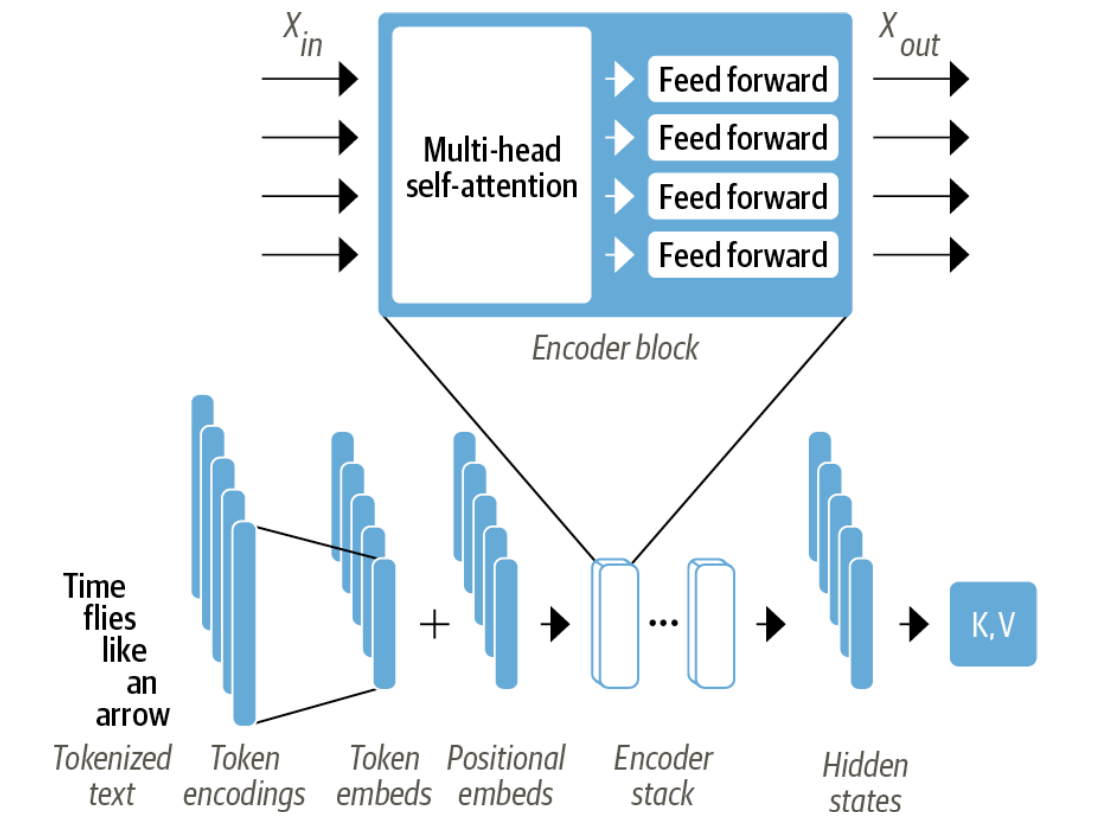
\includegraphics[height=80mm]{graphics/encoder-block.png}
    \caption[Aufbau eines Encoder-Blocks]{Aufbau eines Encoder-Blocks \footnotemark}
    \label{fig:encoder-block}
\end{figure}
\footnotetext{Entnommen aus: \cite{tunstall_natural_2022}, S. 60}
%TODO: Complete Chapter: Decoder, Zusammenspiel, Bottleneck -> Relevanz Attention
Die Mulit-Head Attention Schicht wird im nächsten Abschnitt genauer erläutert. Die Feed-Forward Schicht besteht aus zwei linearen Schichten, welche vollständig miteinander verbunden sind. Die Schichten verarbeiten die Eingabe nicht als ganze Sequenz, sondern die Embeddings unabhängig voneinander. \footcites[Vgl.][S. 70]{tunstall_natural_2022} Die Rolle der Feed-Forward Schicht bleibt im Großteil der Literatur unerwähnt. Jedoch wird durch Geva et. al. die Rolle der Feed-Forward Schicht näher definiert. Es zeigt sich, dass die Feed-Forward Schicht als \emph{key-value memory} funktioniert. Jeder Schlüssel korreliert dabei mit einem menschlich interpretierbaren Eingabemuster. Die Werte erzeugen Verteilungen über den Ausgabewortschatz, die mit der Verteilung des nächsten Tokens von Mustern in dem entsprechenden Schlüssel korrelieren. \footcites[Vgl. dazu ausführlich][S. 5484 ff.]  {geva_transformer_2020} Vereinfacht gesagt hilft das Feed-Forward Netz dem Modell, auf Basis der Eingabedaten die Vorhersagen zu treffen. Die Schlüssel und Werte helfen dem Modell dabei, Muster zu erkennen und mit diesen Mustern verbundene wahrscheinliche Fortsetzungen vorzuschlagen. Die Feed-Forward Schicht ist wichtig, weil sie es Transformern ermöglicht komplexe Datenmuster durch nicht-lineare Transformationen zu lernen und zu interpretieren was entscheiden für die Verarbeitung und das Verständnis von Sprache ist.
Ein entscheidender Nachteil der Encoder-Decoder Architektur ist, dass sie einen Flaschenhals in der Informationsübertragung bildet. Die Eingabe wird in eine einzige Repräsentation umgewandelt, welche dann in den Decoder übergeben wird. Dieser Zustand muss alle Informationen enthalten, die für die Generierung der Ausgabe notwendig sind. \footcites[Vgl.][S. 6 ff.]{tunstall_natural_2022} Diesem Flaschenhals kann durch die Verwendung von \emph{Attention} entgegengewirkt werden. So erhält der Decoder die Möglichkeit auf alle relevanten hidden states des Encoders zuzugreifen, um die Ausgabe zu generieren. \footcites[Vgl.][S. 9]{bahdanau_neural_2014} Eine Erläuterung des Attention-Mechanismus erfolgt in Kapitel 2.2.2.

\paragraph{Decoder:} 
 Wie bereits erwähnt hat der Decoder das Ziel, die Ausgabe zu generieren. Die genaue Struktur des Decoder-Blocks ist in Abb. \ref{fig:decoder-block} dargestellt. Transformer sind in jedem Arbeitsschritt auto-regressiv was bedeutet, dass sie die zuvor generierte Ausgabe als Eingabe für den nächsten Schritt verwenden. In der Abbildung ist zu sehen das diese Eingabe der zu Teilen übersetzte Text aus dem Encoder-Block ist. Diese Eingabe wird in der \emph{Masked multi-head attention} Schicht verarbeitet. Im nächsten Schritt wird die Ausgabe der Masked multi-head attention Schicht samt den hidden states des Encoders in der \emph{Multi-Head Attention} Schicht verarbeitet. Die Ausgabe wird dann in der \emph{Feed-Forward} Schicht verarbeitet. Anschließend wird die Ausgabe der Feed-Forward Schicht in den nächsten Decoder-Block übergeben. \footcites[Vgl.][S. 3 ff.]{vaswani_attention_2017} Dies geschieht solange, bis die Ausgabe vollständig generiert wurde.
 \begin{figure}[h]
    \centering
    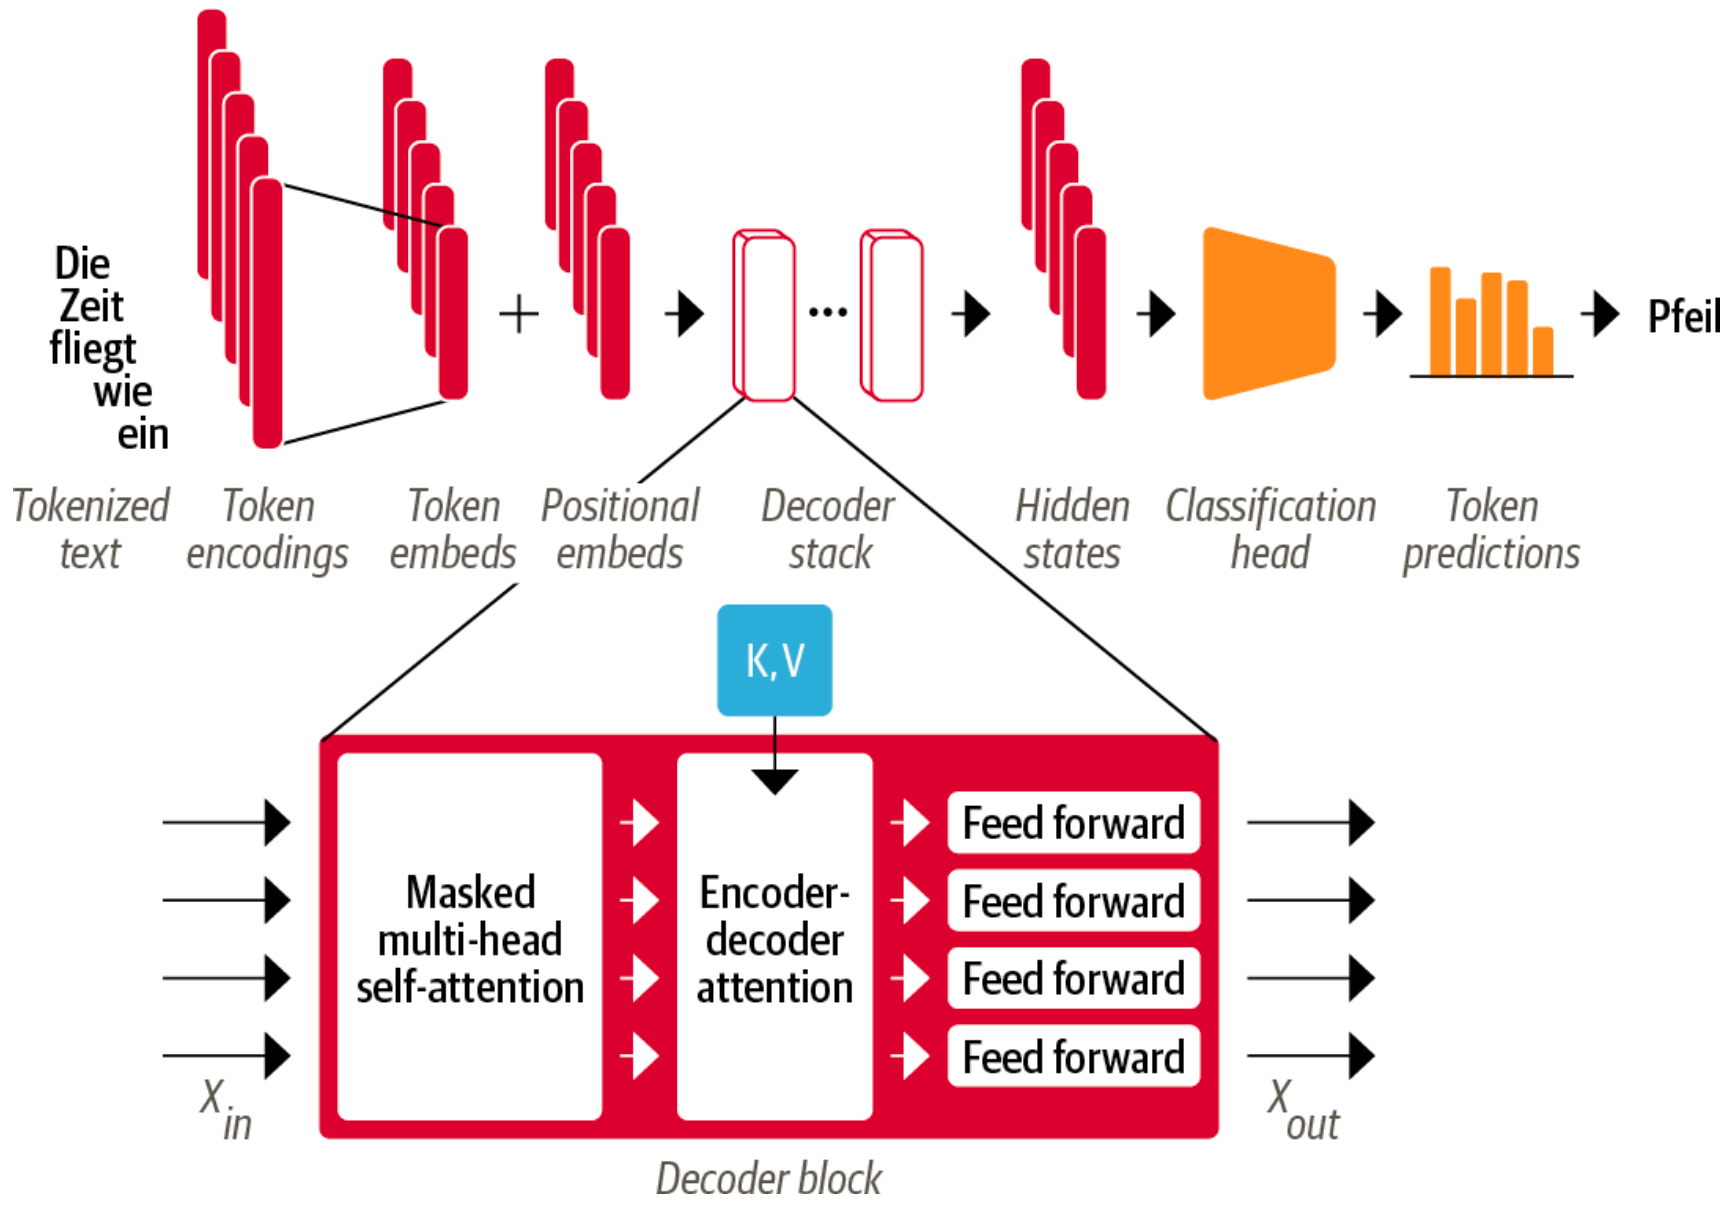
\includegraphics[height=80mm]{graphics/decoder-block.png}
    \caption[Aufbau eines Decoder-Blocks]{Aufbau eines Decoder-Blocks \footnotemark}
    \label{fig:decoder-block}
\end{figure}
\footnotetext{Entnommen aus: \cite{tunstall_natural_2022}, S. 77}

Auch die Interpretation der Funktionsweise des Decoders bleibt in der Literatur weitestgehend unerforscht. Yang et. al. untersuchen die Rolle der Decoder-Schicht und kommen zur Beobachtung, dass der Decoder-Block in drei Aufgabenbereiche eingeteilt werden kann:\footcites[Vgl.][S. 2]{yang_sub-layer_2020}
\begin{enumerate}[1.]
    \item \emph{\ac{TEM}:} Der Decoder nutzt die Informationen des bereits generierten Teils der Ausgabe bzw. der \emph{Zielhistorie} (Output Embeddings s. Abb. \ref{fig:transformer-architecture}) durch die \emph{Masked Multi-Head Attention} Schicht. Er hält die Informationen darüber, was bisher generiert wurde, um eine koheränte Fortsetzung der Zielsequenz zu gewährleisten.
    \item \emph{\ac{SEM}:} Der Decoder wählt relevante Informationen der Quellseite mithilfe der Encoder-Attention (s. Abb. \ref{fig:transformer-architecture} Multi-Head Attention Layer im Decoder) aus, um die Generierung des nächsten Tokens in der Sequenz zu unterstützen. Dies beinhaltet dynamische Aufmerksamkeit auf verschiedene Teile der last hidden states, basierend auf dem aktuellen Zustand der Sequenzgenerierung.
    \item \emph{\ac{IFM}:} Die Informationen aus der Zielhistorie und der Quelleingabe des Encoders werden kombiniert, um die nachfolgenden Ausgabetokens zu generieren. Dieser Teil verschmilzt im Wesentlichen die beiden Informationsströme, um die Generierung der Ausgabe zu unterstützen.
\end{enumerate}
\begin{figure}
    \centering
    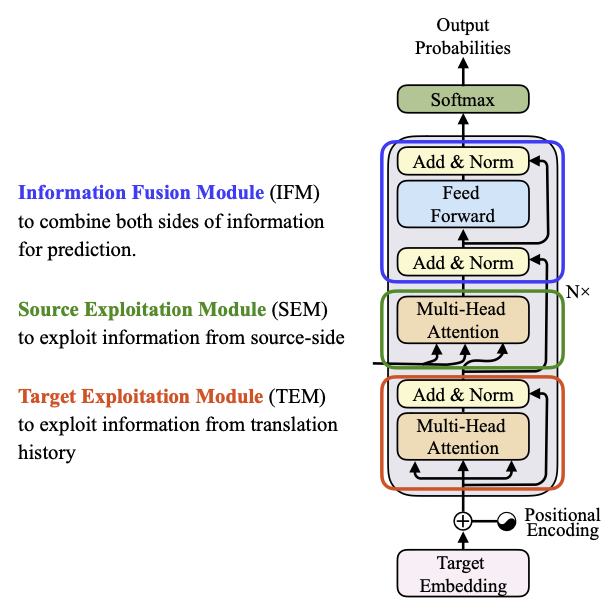
\includegraphics[height=100mm]{graphics/decoder layers explained.png}
    \caption[Aufteilung der Decoder-Schichten in die jeweiligen Funktionen]{Aufteilung der Decoder-Schichten in die jeweiligen Funktionen (\textbf{Lasse ich nur eventuell drinnen, je nachdem ob es wirklich mehrwert bringt und das Springen zwischen Seiten zu viel ist})\footnotemark}
    \label{fig:decoder-layers}
\end{figure}
\footnotetext{Entnommen aus: \cite{yang_sub-layer_2020}, S. 2}

\subsection{Konzepte und Terminologie der Transformer-Modelle}
Das Modell des Transformers basiert auf drei Schlüsselkonzepten: \emph{Self-Attention}, \emph{Multi-Head Attention} und \emph{Positional Encoding}. Diese Konzepte bilden die Grundlage für die Funktionsweise der Transformer-Modelle. \footcites[Vgl.][S. 1]{vaswani_attention_2017} Dieser Abschnitt behandelt die Funktionsweise dieser Konzepte und betrachtet die Anwendung dieser Konzepte in der Architektur der Transformer-Modelle.

Um Self-Attention und Multi-Head Attention verstehen zu können, muss zunächst die Abgrenzung der beiden Begriffe zueinander und zum Begriff \emph{Attention} erfolgen. Der Begriff Attention im Zusammenhang mit künstlicher Intelligenz wird zunächst von Bahdanau et. al. als ein Mechanismus beschrieben, der es Komponenten eines Modells ermöglicht sich auf relevante Teile einer Eingabe zu konzentrieren um eine bestimmte Ausgabe zu erzeugen. \footcites[Vgl.][S. 2 ff.]{bahdanau_neural_2014} Klassische Encoder-Decoder Architekturen tendieren bei langen Eingabesequenzen dazu, die ersten Teile der Eingabe in der Verarbeitung zu vergessen. Dieses Problem wird durch die Verwendung von Attention gelöst. Attention kann bspw. in der Übersetzung von Sätzen verwendet werden, um die Relevanz von Wörtern in der Quellsprache für die Übersetzung in die Zielsprache zu bestimmen. Dies kann in einer Alignment-Matrix dargestellt werden, welche die Relevanz der Wörter in der Quellsprache für die Übersetzung in die Zielsprache darstellt. Hellere Felder deuten dabei auf eine höhere Relevanz in der Verarbeitung hin. Es wird deutlich dass Attention den Fokus auf die Beziehung zwischen unterschiedlichen Sequenzen oder Zuständen in einem Modell legt (hier die Beziehung zwischen dem zu übersetzendem Text und der Übersetzung).\footcites[Vgl.][S. 5 ff.]{bahdanau_neural_2014}
\begin{figure}[h]
    \centering
    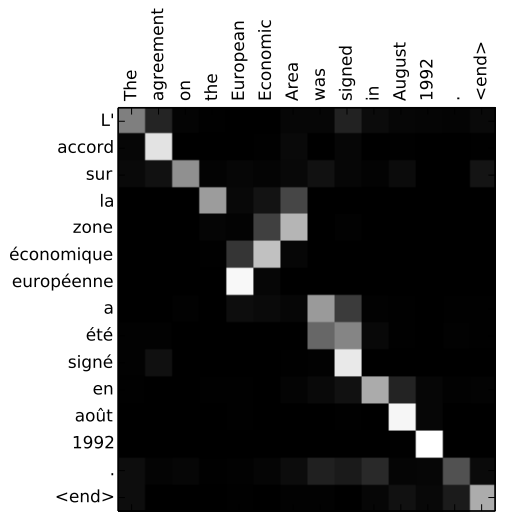
\includegraphics[height=60mm]{graphics/alignment_matrix.png}
    \caption[Alignment-Matrix]{Alignment-Matrix \footnotemark}
    \label{fig:attention}
\end{figure}
\footnotetext{Entnommen aus: \cite{bahdanau_neural_2014}, S. 6}

\textbf{Self-Attention} ist eine spezielle Form der Attention. Der Self-Attention Mechanismus kann Beziehungen zwischen Wörtern über lange Distanzen modellieren \footcites[Vgl.][S. 3]{ramachandran_stand-alone_2019} was dem zuvor erwähnten Flaschenhals im Encoder entgegengewirkt bzw. fast vollständig beseitigt. \emph{Self} bezieht sich dabei auf die Tatsache, dass die Gewichte für alle hidden states im \emph{selben} Block berechnet werden bspw. für alle hidden states innerhalb des Encoder Blocks. Im Gegensatz dazu wird beim Attention-Mechanismus die Relevanz jedes verborgenen Zustands des Encoders für jeden verborgenen Zustand des Decoders zu einem bestimmten Decodierungsschritt berechnet. Self-Attention kann statt eines festen Embeddings für jedes Token die gesamte Sequenz heranziehen, um einen gewichteten Durchschnitt auf Basis der Embeddings zu berechnen. \footcites[Vgl.][S. 61]{tunstall_natural_2022} Warum die Durchschnittsbildung sinnvoll ist, soll folgendes Beispiel verdeutlichen: Das Wort \emph{apple} wird größtenteils mit der Frucht assoziiert. Wenn sich der Kontext ändert, wird ersichtlich, dass es sich dabei eher um das Unternehmen \emph{Apple} handelt wie z. B. in dem Satz \emph{'Apple sold over one million phones and notebooks in the past few months'}. Self-Attention erstellt einen Darstellung des Wortes, welche den Kontext berücksichtigt, indem die Token-Embbedings mit unterschiedlichen Gewichtungen kombiniert werden, etwa indem \emph{Apple} und \emph{notebooks} ein höheres Gewicht zugewiesen wird. Die auf diese Weise erzeugten Embeddings werden Contextualized Embeddings (kontextualisierte Embeddings) genannt. \footcites[Vgl.][S. 1]{peters_deep_2018}

\begin{figure}[h]
    \centering
    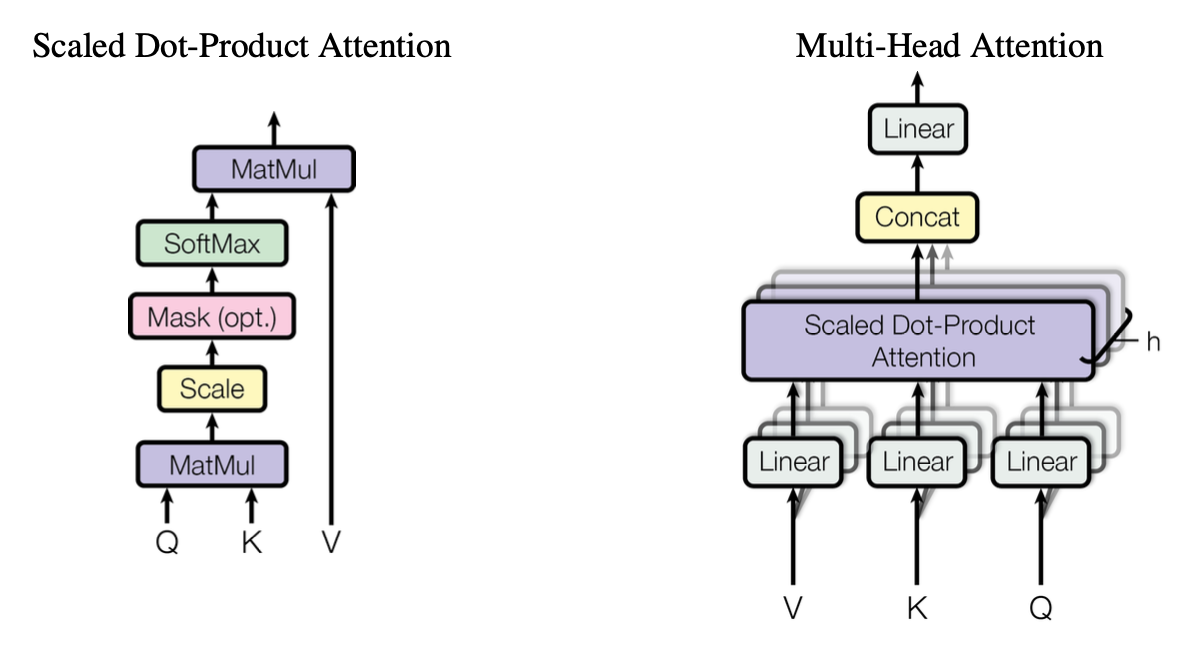
\includegraphics[height=80mm]{graphics/multi-head.png}
    \caption[Aufbau der Scaled Dot-Product Attention und des Multi-Head Attention]{Aufbau der Scaled Dot-Product Attention und des Multi-Head Attention\footnotemark}
    \label{multi-head}
\end{figure}
\footnotetext{Entnommen aus: \cite{vaswani_attention_2017}, S. 4}
Die Attention-Gewichte werden im Transformer über das \emph{Scaled Dot-Product} berechnet (s. Abb. \ref{multi-head}). Alternativ könnten die Attention-Gewichte über additive Attention berechnet werden. Allerdings ist die Leistungsfähigkeit der Scaled Dot-Product Berechnung aufgrund von hochoptimierten Code zur Matrizenmultiplikation deutlich höher. Die Eingabe in das Scaled Dot-Product teilt sich in drei Vektoren auf: \emph{Query, Key und Value}.\footcites[Vgl.][S. 3 f.]{vaswani_attention_2017} Ihre Bedeutung für den Attention-Mechanismus lässt sich wie folgt erklären:\footcites[Vgl.][S. 64]{tunstall_natural_2022}

\begin{itemize}
    \item \textbf{Query:} Die Query (Q) repräsentiert das Element (z. B. ein Wort in einem Satz), für das das Modell den Kontext verstehen möchte. Es ist wie eine Anfrage, die das Modell an alle anderen Wörter im Satz richtet, um herauszufinden, wie relevant sie für das aktuelle Wort sind.
    \item \textbf{Key:} Der Key (K) repräsentiert jedes Element in der Eingabesequenz, gegenüber der die Queries abgeglichen werden. Der Key hilft dem Modell zu entscheiden, wie relevant jedes andere Wort/Element im Kontext des aktuellen Wortes/Elements ist.
    \item \textbf{Value:} Der Value (V) ist der Inhalt/Repräsentation jedes Elements in der Eingabesequenz. Nachdem das Modell mithilfe der Queries und Keys festgestellt hat, wie relevant jedes Element für das betrachtete Element ist, werden die Values gewichtet und aggregiert, um einen neuen Repräsentationsvektor für das betrachtete Element zu erzeugen. Dieser Vektor ist eine Kombination der Informationen, die basierend auf ihrer Relevanz ausgewählt wurden.
\end{itemize}

Zunächst werden die Key und Query Matrizen miteinander multipliziert. Es wird hierbei die Ähnlichkeit zwischen den beiden Matrizen berechnet. Je höher der Score, desto relevanter ist der Key für die Query. Anschließend werden die Werte der Attention Scores skaliert, um große Werte zu vermeiden. Würde dies nicht durchgeführt werden, dann würde die Softmax %TODO: Erklären%
unter Umständen lediglich Werte erzeugen, die ausschließlich sehr nahe gegen 1 oder gegen 0 laufen. \footcites[Vgl. dazu ausführlich][S. 4]{vaswani_attention_2017} Die Maskierung wird in diesem Modell lediglich im Decoder angewandt (s. Abb. \ref{fig:decoder-block}). Der Decoder erhält die Output-Embeddings als neuen Input. Um zu vermeiden, dass dieser in die Zukunft schaut, können noch nicht vorhergesagte Tokens maskiert werden. So bleiben noch nicht erzeugte Tokens dem Modell unbekannt (siehe dazu Anhang x). Die Softmax-Funktion stellt sicher, dass alle Spaltenwerte sich zu 1 aufsummieren lassen. Die entstandene Matrix enthält alle Attention Gewichte. Abschließend wird diese Matrix mit dem Value-Vektor verrechnet. Die Vektoren enthalten nun eine kontextualisierte Repräsentation der ursprünglichen Query, angereichert mit Informationen aus der gesamten Sequenz. \footcites[Vgl.][S. 62 f.]{tunstall_natural_2022}

Dieser Prozess bildet einen \emph{Head} in der Multi-Head Attention. Ein Head ist eine eigenständige Einheit innerhalb des Attention-Mechanismus, die unabhängig Queries, Keys und Values verarbeitet, um eine eigene Version der Attention-Gewichtung zu berechnen. \emph{Multi-Head} meint, dass der Prozess häufiger parallel durchgeführt wird, wobei jeder Head unterschiedliche Aspekte der Daten erfasst, indem er auf verschiedene Repräsentationen der Eingabe arbeitet. \footcites[Vgl.][S. 4 f.]{vaswani_attention_2017} Die Vorteile sind einerseits Diversifizierung, da jeder Head unterschiedliche Beziehungen zwischen den Eingabedaten erfassen kann und andererseits eine reichhaltige Repräsentation. Durch die Kombination der Ergebnisse aus mehreren Heads kann das Modell eine reichhaltigere, multidimensionale Repräsentation von Daten erzeugen, was zu besseren Leistungen bei einer Vielzahl von Aufgaben führt.

Die letzte Besonderheit des Transformers sind die \emph{Positional Encodings}. Da das Modell keine Rekurrenz oder Konvolution verwendet, müssen die Token Embeddings um ihre relative bzw. absolute Position in der Sequenz angereichert werden. Aus diesem Grund werden Positional Embeddings den Token Embeddings hinzugefügt, um die Token Embeddings um Informationen bezüglich ihrer Position in der Sequenz anzureichern. \footcites[Vgl.][S. 6]{vaswani_attention_2017}

\section{Document Understanding Transformer}
Es soll nun dargestellt werden, wie die Transformer in der Dokumentenverarbeitung im Bereich des \ac{VDU} eingesetzt werden. Dazu wird zunächst die Integration der Transformer in die Dokumentenverarbeitung erläutert. Anschließend wird die Funktionsweise des \ac{Donut} genauer betrachtet. Zuletzt werden die Vorteile des \ac{Donut} gegenüber herkömmlichen Methoden dargestellt.

\subsection{Integration von Transformer-Modellen in die Dokumentenverarbeitung}
Wie bereits in Kapitel 2.1 beschrieben, ist die Zusammenarbeit zwischen OCR und künstlicher Intelligenz keine Neuheit. In der Klassifizierungsphase von OCR werden neuronale Netze verwendet, um Inhalte zu klassifizieren. Viele Ansätze der heutigen Literatur verwenden in der Dokumentenverarbeitung ein nachgelagertes Modell zur OCR, welches die Inhalte der OCR weiterverarbeitet. \footcites[Vgl.][]{hwang_post-ocr_2019} \footcites[Vgl.][]{hwang_spatial_2021} \footcites[Vgl.][]{xu_layoutlm_2020} Entsprechend der Beschreibung in Kapitel 2.3 zeigt sich, dass Transformer sehr gut für die Textverarbeitung geeignet sind. \ac{VDU} bzw. \ac{VrDU} geht über die reine Textverarbeitung hinaus. Dieser Aufgabenbereich zielt darauf ab, gescannte oder digitale Unternehmensdokumente (Bilder von Rechnungen, Formulare im PDF-Format etc.) mit strukturierten Informationen automatisch zu extrahieren und zu organisieren. \ac{VrDU} benötigt dabei nicht nur textuelle Informationen, sondern auch visuelle und layoutbasierte Information, die kritisch für \ac{VrDU} sind. \footcites[Vgl.][S. 1192]{xu_layoutlmv2_2022} Beispielsweise ist bei einer Rechnung die Position des Einzelpreises in der Spalte \emph{Einzelpreis} wichtig, damit diese nicht irrtümlich als Gesamtpreis verarbeitet wird. Das heißt, dass ein Transformer wie bspw. BERT nicht zwingend ohne Weiteres für die Verarbeitung für layoutbasierte Dokumente geeignet ist. Die Embeddings in den Transformern müssen daher um zusätzliche Informationen angereichert werden. Vorherige Ansätze im Bereich des \ac{VDU} verwendeten konvolutionale Netze (\ac{CNN}), um layoutbasierte Dokumente zu verarbeiten. Allerdings haben diese zwei Mängel: \footcites[Vgl.][S. 1193]{xu_layoutlm_2020}
\begin{enumerate}[1.]
    \item Sie sind von einigen wenigen von Menschen annotierten Trainingsdaten abhängig.
    \item Sie verwenden vortrainierte NLP-Modelle, jedoch lassen sie ein gemeinsames Training von textuellen und layoutbasierten Informationen außer acht.
\end{enumerate}
Modelle wie LayoutLM wirken diesen Problemen entgegen indem zwei weitere Input Embeddings im Training verwendet werden. Einerseits ein 2-D Position Embedding, welches die relative Postition eines Wortes in einem Dokument annotiert und andererseits ein Image Embedding für gescannte und tokenisierte Bilder in einem Dokument. \footcites[Vgl.][S. 1193]{xu_layoutlm_2020} Auf diese Weise können Transformer-Modelle in die Dokumentenverarbeitung integriert werden. \ac{SOTA}-Modelle wie LayoutLMv3\footcites[Vgl. dazu ausführlich][]{huang_layoutlmv3_2022}, Ernie\footcites[Vgl. dazu ausführlich][]{peng_ernie-layout_2022} oder FastStrucText\footcites[Vgl. dazu ausführlich][]{zhai_fast-structext_2023} bauen auf diesen Grundlagen auf und erzielen sehr gute Ergebnisse in der Dokumentenverarbeitung.
\subsection{Unterschiede und Vorteile des Donut}
%TODO: In diesem Abschnitt die Kritische Distanz prüfen: Werden die Probleme von anderen Papern auch so benannt oder ist das nur ein Donut-Ding?
Die zuvor beschriebenen OCR-abhängigen Modelle haben trotz ihrer guten Ergebnisse in der Dokumentenverarbeitung einige Probleme. Die Vorverarbeitung ist sehr aufwendig. Es können zwar schon vortrainierte OCR Systeme verwendet werden, allerdings würde der Rechenaufwand für die Inferenz zu hoch sein, um hochqualitative Ergebnisse zu erzielen. Des Weiteren haben OCR-abhängige Ansätze selten die Flexibilität, um unterschiedliche Sprachen oder Dokumentenbereiche zu verarbeiten, was zu einer mangelhaften Generalisierungsfähigkeit führen kann. Ferner braucht das Training eines OCR-Modells eine große Menge an Datensätzen. Nicht zuletzt würden Fehler seitens der OCR in das \ac{VDU}-System propagieren. \footcites[Vgl.][S. 2]{kim_ocr-free_2021} Ein 
%TODO: Schreiben, dass Donut die Probleme löst, aber durchaus zu beachten ist, dass XYLayoutLM diese Ebenfalls annerkennt aber auch angeht. Hier sagen, dass Donut nicht als einzige Lösung gesehen werden soll, sondern als eine von vielen.
Donut zielt darauf ab, diese Herausforderungen zu überwinden. Vorteil von Donut ist hierbei, dass auf layoutbasierte Informationen wie bspw. die Koordinaten der erkannten Felder bei der Datenanotation vollständig verzichtet werden kann. Im Gegensatz zu herkömmlichen Methoden, die sich auf externe OCR-Engines verlassen, modelliert Donut eine direkte Abbildung vom rohen Eingabebild zum gewünschten Ausgabeformat ohne die Verwendung von OCR. Diese Herangehensweise bietet mehrere entscheidende Vorteile:\footcites[Vgl.][S. 3]{kim_ocr-free_2021}
\begin{itemize}
    \item Reduzierte Rechenkosten: Donut eliminiert die Notwendigkeit, externe OCR-Engines als Vorverarbeitungsschritt einzusetzen, wodurch die Gesamtrechenkosten gesenkt werden können.
    \item Erhöhte Flexibilität: Durch den Verzicht auf externe OCR-Modelle erhöht Donut die Flexibilität im Umgang mit verschiedenen Sprachen und Dokumentenformaten. Dies wird weiter durch die Verwendung eines synthetischen Datengenerators unterstützt, der das Pre-Training des Modells in verschiedenen Sprachen und Domänen erleichtert.
    \item Vermeidung von OCR-Fehlerfortpflanzung: Da Donut nicht auf OCR-Ergebnisse angewiesen ist, werden die Probleme der Fehlerfortpflanzung, die sich negativ auf nachfolgende Verarbeitungsschritte auswirken können, vermieden. Dies ist besonders vorteilhaft bei Sprachen mit komplexen Zeichensätzen, wo die OCR-Qualität tendenziell geringer ist.
    \item Verbesserte Genauigkeit und Effizienz: Donut erreicht durch ein einfaches, aber effektives Pre-Training und Fine-Tuning-Schema, das direkt auf Dokumentbildern und deren Textannotationen basiert, eine verbesserte Genauigkeit und Effizienz bei der Verarbeitung visueller Dokumente.
\end{itemize}
Die genannten Vorteile sind jedoch kritisch zu betrachten. Einerseits wurde das Donut-Modell nach Kim et. al. auf unterschiedlichen Benchmark-Datensätzen getestet. Im Unternehmensumfeld können sich die zu verarbeitenden Daten jedoch stark von den Benchmark-Datensätzen wie \ac{FUNSD} oder \ac{CORD} unterscheiden. Donut zeigt gute Ergebnisse bei Daten, welche den Trainingsdaten ähneln. Bei komplexen Dokumenten wie InfoVQA\footcites[Vgl. dazu ausführlich][]{mathew_infographicvqa_2021} sind die Ergebnisse schlechter.\footcites[Vgl.][S. 693]{aggarwal_dublin_2023} Andererseits ist zu beachten, dass OCR-freie Ansätze nicht als einzige Modelle die Probleme der OCR-Abhängigkeit lösen. LayoutLMv3 und FastStrucText sind ebenfalls OCR-freie Ansätze, die die Probleme der OCR-Abhängigkeit anerkennen und angehen. \footcites[Vgl. dazu ausführlich][]{huang_layoutlmv3_2022} \footcites[Vgl. dazu ausführlich][]{zhai_fast-structext_2023} Donut sollte daher nicht als einzige Lösung gesehen werden, sondern als eine von vielen. Diese kritische Betrachtung wird in dieser Arbeit genauer dargestellt, da einerseits Datensätze aus dem Unternehmensumfeld verwendet werden und andererseits die Ergebnisse von Donut mit anderen OCR-abhängigen Ansätzen wie bspw. LayoutLMv3 verglichen werden.

\subsection{Architektur des Donut}
Die Architektur von Document Understanding Transformer (Donut) repräsentiert einen signifikanten Fortschritt in der automatisierten Verarbeitung visueller Dokumente. Donut unterscheidet sich grundlegend von OCR-abhängigen Modellen durch seinen End-to-End-Ansatz, der das direkte Verstehen von Dokumentbildern ermöglicht, ohne auf herkömmliche OCR-Techniken angewiesen zu sein. Im Folgenden wird die Architektur des Donut skizziert und den OCR-abhängigen Modellen gegenübergestellt, um ein Verständnis für das Modell gegenüber traditionelle Ansätzen zu schaffen.

Die Grundlage von Donut bildet eine Transformer-basierte Architektur, die in zwei Hauptkomponenten unterteilt ist: einen visuellen Encoder und einen textuellen Decoder.\\
\textbf{Visueller Encoder:} Der visuelle Encoder von Donut transformiert Eingabedokumentbilder in eine Menge von Embeddings, die visuelle Merkmale des Dokuments repräsentieren. Diese Embeddings dienen als Basis für das Verständnis der strukturellen und inhaltlichen Aspekte des Dokuments.\footcites[Vgl.][S. 4]{kim_ocr-free_2021}\\
\textbf{Textueller Decoder:} Der Decoder nutzt die vom Encoder generierten Embeddings, um eine Sequenz von Token zu generieren, die den im Dokument enthaltenen Text sowie dessen Layout und Struktur widerspiegeln. Diese Token-Sequenz kann dann in ein gewünschtes strukturiertes Ausgabeformat, wie z.B. \ac{JSON} konvertiert werden, das die extrahierten Informationen organisiert.\footcites[Vgl.][S. 5]{kim_ocr-free_2021}

\begin{figure}[]
    \centering
    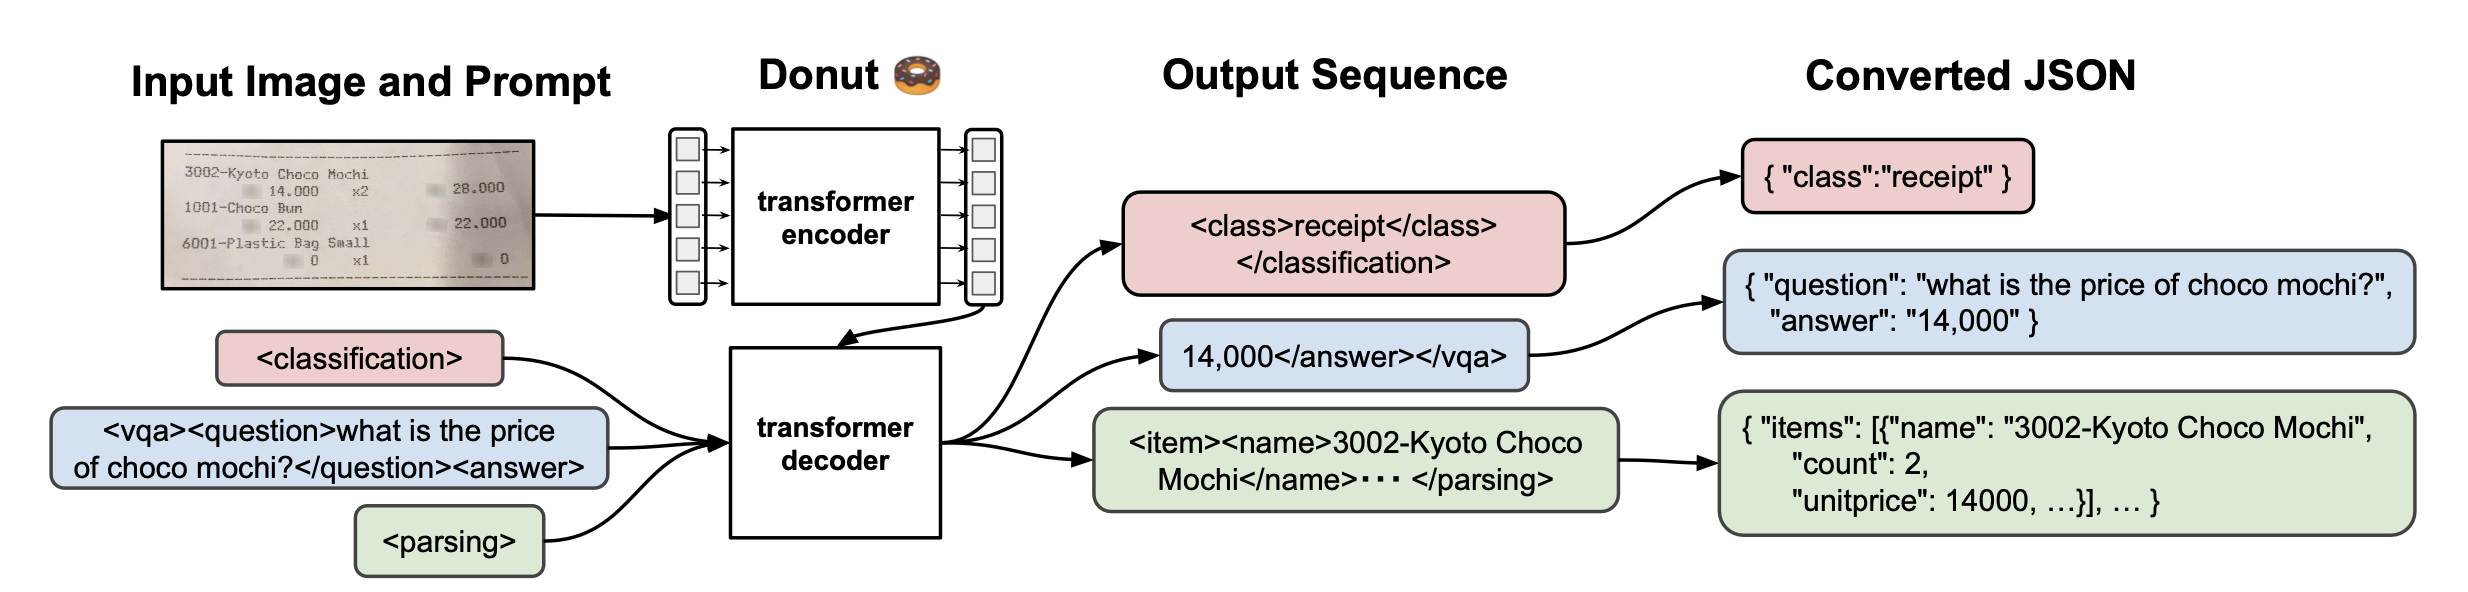
\includegraphics[width=160mm]{graphics/donut-architecture.png}
    \caption[Architektur des Donut]{Architektur des Donut\footnotemark}
    \label{fig:donut-architecture}
\end{figure}
\footnotetext{Entnommen aus: \cite{kim_ocr-free_2021}, S. 4}
Abb. 8 soll den Aufbau verdeutlichen. Auf Basis dieser Architektur können Dokumente klassifiziert werden. Des Weiteren können Fragen zum Dokument beantwortet werden. Für die Implementierung in einer Endanwendung ist das Parsing/Extraktion von besonders hoher Bedeutung, da das Dokument in ein strukturiertes Format wie bspw. \ac{JSON} umgewandelt werden kann. Dieses kann anschließend durch Drittanwendungen weiterverarbeitet werden. 

OCR-abhängige Modelle folgen einem zweistufigen Prozess: Zuerst wird OCR verwendet, um Text aus dem Dokumentbild zu extrahieren. Anschließend werden die OCR-Ergebnisse in einem separaten Schritt verarbeitet, um die Dokumentstruktur und den Inhalt zu verstehen und zu organisieren. Im Gegensatz dazu integriert Donut das Lesen und Verstehen von Dokumenten in einem einzigen, einheitlichen Prozess. Dieser End-to-End-Ansatz kann zu den in Kapitel 2.3.2 beschriebenen Vorteilen führen. Abb. 9 stellt die Unterschiede nochmals dar. \footcites[Vgl.][S. 2 f.]{kim_ocr-free_2021}
\begin{figure}[h]
    \centering
    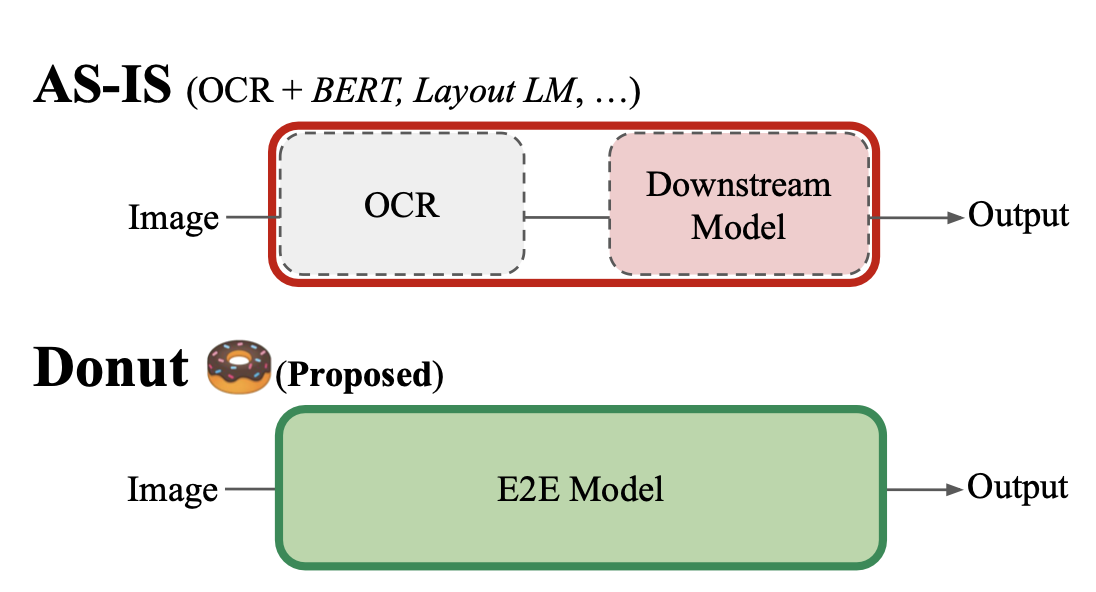
\includegraphics[height=40mm]{graphics/e2e.png}
    \caption[Vergleich der Pipelines]{Vergleich der Pipelines\footnotemark}
    \label{fig:pipelines}
\end{figure}
\footnotetext{Entnommen aus: \cite{kim_ocr-free_2021}, S. 2}

\section{Bestehende Forschung zu OCR-abhängigen Modellen in der Dokumentenverarbeitung}
Zur Zeit gibt es eine Vielzahl von Forschungspapieren, die sich mit der Dokumentenverarbeitung beschäftigen. Einige davon untersuchen OCR-abhängige Ansätze und versuchen diese zu verbessern. Andere setzen auf OCR-freie Ansätze wie Donut. In den folgenden beiden Kapiteln werden einige wichtige Ergebnisse aus der Literatur vorgestellt und kritisch betrachtet. Dies soll ein umfassendes Verständnis für die aktuellen SOTA-Modelle schaffen und die Relevanz anderer Modelle für Unternehmen darstellen.

Im Bereich der OCR-abhängigen Ansätze sind v. a. vier Modelle von Bedeutung: OCR + Bert, LayoutLMv3 (aber auch die Derivate), Ernie und FastStrucText. Diese Modelle haben in den letzten Jahren die SOTA-Modelle in der Dokumentenverarbeitung dargestellt. Im folgenden werden die Forschungsergebnisse dieser Modelle zusammengefasst und kritisch betrachtet.

\textbf{OCR + Bert (August 2020):} Der Ansatz einen Transformer der OCR nachzuschalten bildet die Grundlage für alle weiteren betrachteten Modelle in diesem Kapitel.Das Modell OCR + BERT konzentriert sich auf die Nachbearbeitung von durch OCR generiertem Text, um Fehler zu erkennen und zu korrigieren. Diese Methode kombiniert das \ac{BERT}-Modell mit Techniken der \ac{NMT}, um fehlerhafte Tokens zu identifizieren und zu korrigieren. Die Verwendung von BERT ermöglicht es, den Kontext von Wörtern zu berücksichtigen, was insbesondere bei der Korrektur von kontextabhängigen Fehlern hilfreich ist. Die Kombination aus BERT und NMT zielt darauf ab, die Genauigkeit des durch OCR erzeugten Textes zu verbessern, indem sowohl offensichtliche als auch subtilere Fehler, die durch OCR-Technologien verursacht werden, angegangen werden.\\
In einer Studie, die die Effektivität dieser Methode bewertet, zeigen die Ergebnisse, dass der Ansatz vergleichbare oder sogar bessere Leistungen im Vergleich zu den besten existierenden Methoden für die Nachbearbeitung von OCR-Text erbringt. Diese Ergebnisse wurden insbesondere durch die Teilnahme an den Wettbewerben zur Post-OCR-Textkorrektur in den Jahren 2017 und 2019 (ICDAR) erzielt, wo das OCR + BERT-Modell ähnliche oder leicht verbesserte Ergebnisse im Vergleich zu den Gewinnern dieser Wettbewerbe erzielte. Besonders hervorzuheben ist die Fähigkeit des Modells, nicht nur nicht-wortbasierte Fehler zu erkennen und zu korrigieren, sondern auch kontextabhängige Fehler, die eine größere Herausforderung darstellen, effektiv zu adressieren. Die Kombination aus BERT für die Fehlererkennung und NMT für die Fehlerkorrektur bietet einen vielversprechenden Ansatz zur Verbesserung der Textqualität von durch OCR digitalisierten Dokumenten. Durch die Berücksichtigung des Kontexts und die Fähigkeit, sowohl einfache als auch komplexe Fehler zu korrigieren, stellt dieser Ansatz einen bedeutenden Fortschritt in der Post-OCR-Textbearbeitung dar. \footcites[Vgl. dazu ausführlich][S. 335 ff.]{nguyen_neural_2020}

\textbf{LayoutLMv3 (April 2022):} LayoutLMv3 erweitert die Fähigkeiten seiner Vorgänger durch die Integration von Bild- und Textmerkmalen innerhalb eines einheitlichen Transformer-Modells, das sowohl Selbst- als auch Kreuzmodalitätsaufmerksamkeitsmechanismen verwendet. Dies ermöglicht eine effektive Handhabung der räumlichen Anordnung von Textelementen und deren visuellen Kontext, was zu einer verbesserten Leistung bei der Dokumentenverarbeitung führt. LayoutLMv3 zeigt bemerkenswerte Ergebnisse in verschiedenen Benchmarks zur Dokumentenverständnis, darunter Formularverstehen und Informationsentnahme aus komplexen Layouts. Besonders nennenswert ist das Ergebniss von LayoutLMv3-Base im Vergleich zu BERT und DocFormer (ein E2E-Ansatz, welcher aber noch von OCR abhängig ist). LayoutLMv3-Base erzielt in den Benchmarks zu \ac{FUNSD} und \ac{CORD} respektive einen F1-Score von 90.29 \% und 96.56 \%. BERT hingegen erzielt jeweils 60.26 \% und 89.68 \% und DocFormer 83.34 \% und 96.33 \%. LayoutLMv3-Base stellt daher eine potenzielle Alternative zu OCR-freien Modellen dar. \footcites[Vgl. dazu ausführlich][S. 4087 ff.]{huang_layoutlmv3_2022}

\textbf{ERNIE-Layout (Oktober 2022):} ERNIE-Layout nutzt eine fortschrittliche Verarbeitung von visuellen, textuellen und Layoutinformationen, um ein tiefgreifendes Verständnis von Dokumenten zu erzielen. Durch die Einbindung von visuellen Merkmalen direkt in den Transformer-Encoder ist ERNIE-Layout in der Lage, komplexe Zusammenhänge zwischen Textinhalten und ihrem visuellen Kontext effizient zu erfassen. Diese ganzheitliche Betrachtung führt zu einer verbesserten Performance bei der Erkennung und Klassifizierung von Dokumentelementen über ein breites Spektrum von Layouts hinweg. ERNIE-Layout demonstriert seine Wirksamkeit durch herausragende Ergebnisse in verschiedenen Benchmark-Tests, die seine Fähigkeit unterstreichen, präzise Informationen aus visuell reichen Dokumenten zu extrahieren. Es ist jedoch anzumerken, dass ERNIE-Layout-Large lediglich im FUNSD-Benchmark um 1.4 \% besser abschneiden konnte als LayoutLMv3-Large. Im CORD-Vergleich schneidet LayoutLMv3 besser ab als ERNIE, obwohl es sich bei ERNIE um das jüngere Modell handelt. \footcites[Vgl. dazu ausführlich][S. 7 f.]{peng_ernie-layout_2022}

\textbf{FastStrucText (Mai 2023):} Fast-StrucText stellt einen bedeutenden Fortschritt dar, indem es eine effiziente Transformer-Architektur mit einer modality-guided dynamic token merge Technik kombiniert. Dieser Ansatz ermöglicht es, die Anzahl der zu verarbeitenden Tokens dynamisch zu reduzieren, wodurch die Effizienz ohne Einbußen bei der Leistung erhöht wird. Fast-StrucText erreicht eine überlegene Balance zwischen Inferenzgeschwindigkeit und Genauigkeit, indem es die Fähigkeit zur Verarbeitung multi-granularer Repräsentationen optimiert und gleichzeitig den Rechenaufwand minimiert. Die experimentellen Ergebnisse zeigen, dass Fast-StrucText im Vergleich zu bestehenden Methoden eine hohe Leistung aufweist und gleichzeitig eine schnellere Inferenzzeit bietet. Dieser Ansatz stellt daher eine vielversprechende Lösung für die effiziente Verarbeitung visueller Dokumente dar. \footcites[Vgl. dazu ausführlich][]{zhai_fast-structext_2023}

Zusammenfassend zeigen die Ergebnisse, dass OCR-abhängige Modelle wie LayoutLMv3 und ERNIE-Layout weiterhin eine wichtige Rolle in der Dokumentenverarbeitung spielen. Diese Modelle erzielen hervorragende Ergebnisse in verschiedenen Benchmarks und bieten eine effektive Möglichkeit, visuelle Dokumente zu verstehen und zu verarbeiten. Andererseits zeigen OCR-freie Ansätze wie Donut, dass es möglich ist, die OCR-Abhängigkeit zu überwinden und eine effiziente Verarbeitung visueller Dokumente zu erreichen. Das folgende Kapitel widmet sich der Forschungsergebnisse zu OCR-freien Ansätzen.

\section{Bestehende Forschung zu OCR-freien Modellen in der Dokumentenverarbeitung}
Dieses Kapitel stellt die aktuellen Forschungsergebnisse im Bereich der OCR-freien Modelle wie Donut und Dublin dar. Es soll gezeigt werden, wie diese Modelle auch ohne eine vorgelagerten OCR-Komponente \ac{SOTA}-Ergebnisse in der Datenextraktion erzielen. Die Ergebnisse dieser Modelle werden kritisch betrachtet und mit den Ergebnissen der OCR-abhängigen Modelle verglichen.

\textbf{Donut (November 2021):} Das Donut-Modell wurde erstmals im November 2021 vorgeschlagen. Daher ist es jünger als das LayoutLMv3 weshalb die Vergleiche der Experimente im entsprechenden Paper zu LayoutLMv2 gezogen wurden. Da sich diese Arbeit auf den Bereich der Informationsextraktion aus Dokumenten fokussiert sollen die Ergebnisse in den Bereichen Document Classification und Document visual question answering nicht weiter betrachtet werden. Donut zeigt in den Experimenten eine hohe Genauigkeit bei der Extraktion von Informationen aus Dokumenten. Im Vergleich zu LayoutLMv2 erzielt Donut im Benchmark zu \ac{CORD} deutlich bessere Ergebnisse. Die genaue gegenüberstellung der Ergebnisse zeigt Tab. 1. Zu beachten ist jedoch, dass im \ac{CORD}-Benchmark wesentlich schlechter abschneidet als LayoutLMv3 in Bezug auf den F1-Score.\footcites[Vgl.][S. 10]{kim_ocr-free_2021} Allerdings ist anzumerken, dass hier auch der abweichende Versuchsaufbau der Experimente eine Rolle spielen kann. Die Tabellenbeschreibung trägt den Namen: \emph{"Performances on various document IE tasks"}\footcites[][S. 10]{kim_ocr-free_2021} Der genaue Versuchsaufbau ist jedoch nicht bekannt. Von daher sind die Gegenüberstellungen der Ergebnisse in Tab. 1 kritisch zu betrachten.

\textbf{DUBLIN (Mai 2023):} \ac{DUBLIN} ist ein weiteres weitaus jüngeres OCR-freies Modell, welches im Mai 2023 vorgestellt wurde. DUBLIN hat eine ähnliche Architektur zu Donut, jedoch sind Ergebnisse im Vergleich zu Donut deutlich besser. DUBLIN erzielt im \ac{CORD}-Benchmark einen F1-Score von 97.1 \%. Im \ac{FUNSD}-Benchmark erzielt es dennoch lediglich einen F1-Score von 77.8 \%. Im Vergleich zu Donut erzielt \ac{DUBLIN} jedoch deutlich bessere Ergebnisse. Es gibt für unterschiedliche Aufgaben speziallisierte \ac{SOTA}-Modelle die in den jeweiligen Aufgaben abschneiden. Trotzdem sind die Ergebnisse häufig nur marginal besser. Der entscheidende Nachteil ist, dass für jede Aufgabe ein anderes Modell benötigt wird. \ac{DUBLIN} hat den Vorteil, dass es auf ein weites Spektrum von Aufgaben angewandt werden kann. \footcites[Vgl. dazu ausführlich][S. 698]{aggarwal_dublin_2023}

\begin{table}[htbp]
    \centering
    \begin{tabular}{lcccccc}
      \toprule
      & \textbf{LayoutLmV3} & \textbf{FastSrucText} & \textbf{BERT} & \textbf{Donut} & \textbf{DUBLIN} \\
      \midrule
      \textbf{FUNSD} \\
      F1 Score & 90.29 & 90.35 & 60.26 & - & 77.8 \\
      \addlinespace
      \textbf{CORD} \\
      F1 Score & 96.59 & 97.15 & 89.68 & 84.1 & 97.1 \\
      \bottomrule
    \end{tabular}
    \caption{Vergleich der Ergebnisse der Modelle. Es ist anzumerken, dass die OCR-abhängige Modelle im FUNSD-Benchmark deutlich bessere Ergebnisse liefern.}
  \end{table}

  Einige Eigenschaften der Forschung sind hierbei noch kritisch hervorzuheben. Zum einen zeigen diverse Paper die \ac{BERT} in ihren Forschungen vergleichen recht starke Schwankungen. Dies kann unter anderem auf die jeweils verwendete OCR-Engine zurückgeführt werden, durch welche die Qualität der Ergebnisse schon im Vorhinein stark beeinflusst werden kann. Zum anderen ist zu beachten, dass die Ergebnisse aus Benchmarks stammen. Bei \ac{FUNSD} und \ac{CORD} handelt es sich jeweils um einen ganz spezifischen Typ von Daten. Das solche Datensätze zur Bemessung der Modelle benutzt werden erhöht durch die Standardisierung zwar die Vergleichbarkeit der Modelle, jedoch sind die Ergebnisse nicht auf andere Datensätze übertragbar. Es kann auch sein, dass bei sehr heterogenen Rechnungen einige Modelle in der Lage sind, besser abzuschneiden als andere. Dies bekräftigt nochmals die Aufgabe dieser Arbeit, die Ergebnisse der OCR-abhängigen Modelle mit den OCR-freien Modellen zu vergleichen und zu bewerten, v.a. in Bezug auf die Anwendbarkeit in Unternehmen wo Daten nicht zwingend denen der Daten in \ac{FUNSD} oder \ac{CORD} entsprechen. Diese ist vor allem wichtig, da die annotation von Trainingsdaten für das Finetuning von Modellen sehr aufwendig sein kann. Nicht zwingend werden Unternehmen die Ressourcen haben, um solche Datensätze zu erstellen, v.a. solche die den Datensätzen in der Forschung entsprechen. Die Qualität der Trainingsdaten kann sich daher stark auf die Ergebnisse der Modelle auswirken.